\section{Optimizations}

\subsection{File Loading}
When loading a data resource, the greatest bottleneck lies in fetching from a persistent storage medium.
Doing multiple IO operations on a hard disk for example, can heavily increase the load time of a file
due to their mix with other IO operations from the rest of the Operating System\footnote{Programs do
not have exclusive ownership of the hard disk in a multitasking environment}. Having that in mind, resources
from Hard Drive or other persistent storages are best loaded with the fewest IO operations that can be done.
In this case, files are being read in a single shot.

\subsection{Rendering State Changes Minimization}
Often alteration of the driver state (through OpenGL calls for example), may result in stealing precious time
from the program. This occurs because a possible driver call might change the state in our graphics card hardware
or not depending on the action we took.\footnote{Although, modern drivers often try to defer as much state change as
possible till the next draw call} Therefore, redundant graphics API calls are avoided and similar ones are batched
as much as possible.

\subsection{Deferred Rendering}
With the traditional Forward Rendering pipeline, each vertex passes through the GPU processing pipeline regardless
if it is visible or not in the end. That means that lots of fragments reach the final shading stage without even
being visible. In addition, this approach does not scale well with more lights because the more lights there are,
the more unnecessary shading operations are required. This rendering overhead can be avoided by developing a way
to shade only the final visible fragments. This is achieved through a ``Deferred Rendering'' pipeline that is
composed in 2 main passes:

\begin{enumerate}
\item Geometry Pass
\item Lighting Pass
\end{enumerate}

\subsubsection{Geometry Pass}

\begin{figure}[ht]
    \centering
    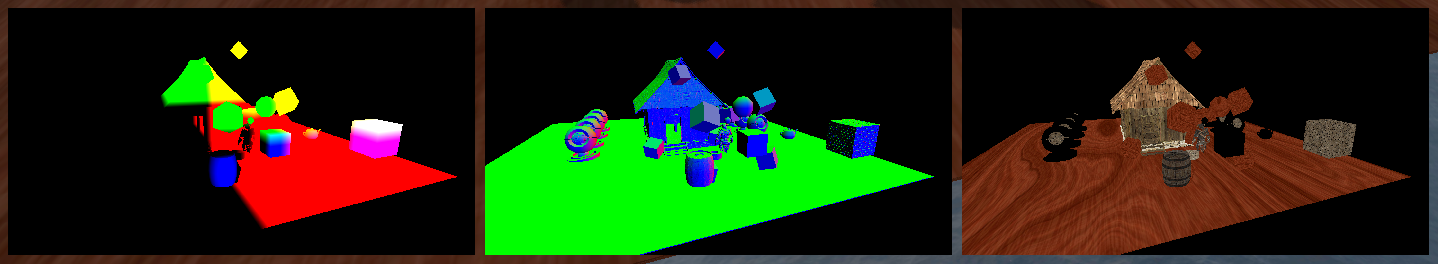
\includegraphics[scale=0.3, clip=true]{./image/gbuffer.png}
    \caption{Position, Normal and BaseColor GBuffer textures}
\label{fig:gbuf}
\end{figure}

In the Geometry Pass  each object is rendered once. Base color, metalness, roughness, reflectivity, and world
space normals are rendered into framebuffer targets (textures) for each final fragment. This logical grouping of
textures is called GBuffer (Geometry Buffer). The GBuffer is set as a Multiple Render Target output in the Geometry
Pass, so in the end of the fragment shading stage all data mentioned above are saved to their respective texture
in the GBuffer which, in turn is bound and used when shading the given fragment in the Lighting Pass. The visualized
contents of some GBuffer textures can be seen in figure~\ref{fig:gbuf}.

\subsubsection{Lighting Pass}

The lighting pass consists of multiple individual light passes; one per direct light plus one for the
environmental lighting. For each sub-pass the lighting for each screen spce fragment is computed, using data from
the GBuffer and bound ShadowMaps. Starting with an empty accumulation texture buffer (black) the final light
contribution from every pass is added. For directional lights and environmental lighting a full screen quad render
is performed, while for point lights only fragments of the area they affect are being rendered.

\begin{figure}[h]
    \centering
    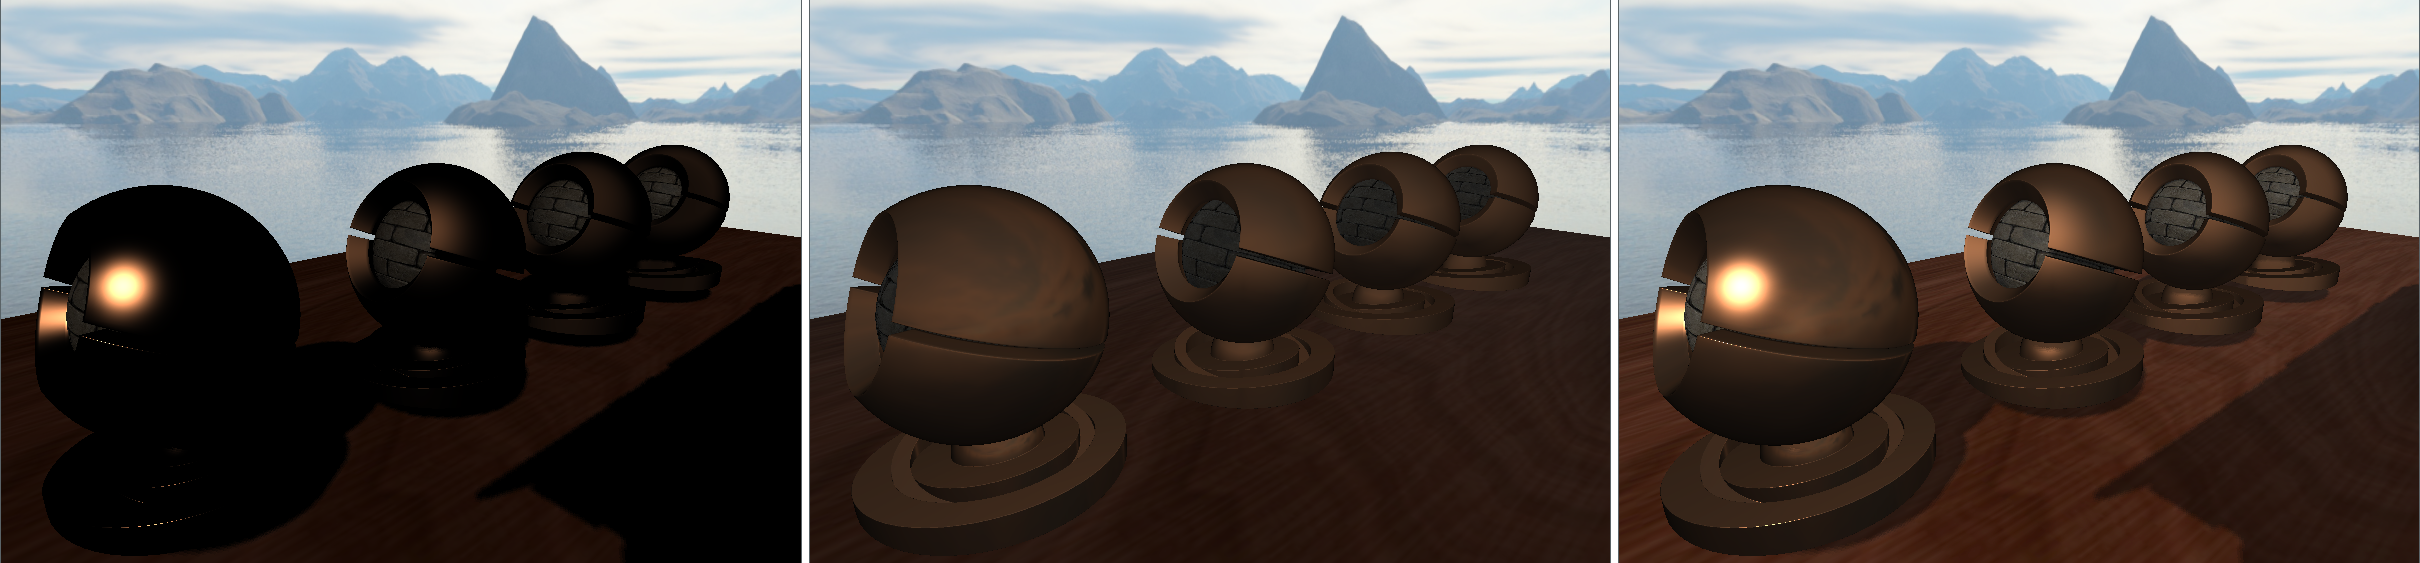
\includegraphics[scale=0.18, clip=true]{./image/lightpasses.png}
    \caption{Directional light, Environmental light and Accumulated light}
\label{fig:lpasses}
\end{figure}

\subsection{Bounding Spheres Optimization}

When making the point light passes it is desirable that we shade only the visible fragments that reside inside the light
source's volume of effect; light from emitters attenuates and contributes negligibly to distant
surface points. Therefore, only points within a certain radius from the (point) light source
center need to be evaluated for lighting, saving significant shading time.
The first attempt on this would be the rendering of a sphere around the point light position instead
of a screen quad pass. The problems with this simplistic approach are directly noticeable:
First, the screen projection of a sphere is a two-dimensional (screen x, y) ellipsoid, preventing
the culling of fragments beyond its z-extents.
Second as soon as the camera center of projection enters the light volume the point light disappears
due to the back face culling being enabled. Disabling back face culling would not be a viable option
as this leads to increased light when outside the sphere (because we render both faces) and inverse
of the original effect if only front face culling is enabled (light only when inside the volume).
To bypass these problems a smart trick using the stencil buffer can be used. It can be separated in two main parts:
\begin{enumerate}
    \item Mark affected fragments in the Stencil Buffer
    \item Render sphere with Stencil Test enabled
\end{enumerate}
In order to mark the affected fragments in the Stencil Buffer we rely on the fact that when we look on the bounding
sphere from the camera point of view:
\begin{enumerate}
    \item Both bounding sphere's front and back face polygons are behind an object that is in front of it
    \item Both bounding sphere's front and back face polygons are in front of an object that is behind it
    \item The front face polygons are in front of but the back face polygons are behind an object that is inside the bounding sphere
\end{enumerate}
So in order to use this with the Stencil Buffer we take the following steps:
\begin{enumerate}
    \item Disable writing into the depth buffer, making it read-only
    \item Disable back face culling, in order to process all the polygons of the sphere
    \item Set the stencil test to always succeed (What we really care is the operation)
    \item Configure the stencil operation for back facing polygons to increment the value in the stencil buffer
        when the depth test fails but keep it unchanged when either depth test or stencil test succeeds
    \item Configure the stencil operation for front facing polygons to decrement the value in the stencil buffer
        when the depth test fails but keep it unchained when either depth test or stencil test succeeds
    \item Render the light sphere using null shaders and disabled output to affect only stencil buffer
\end{enumerate}
This way when an object is outside the bounding volume the stencil buffer is balanced out by the decrement of the
front face polygons and the increment of the back face polygons of the bounding sphere. The result is a stencil buffer
with non zero parts of the object fragments that are affected by the light. Using this the point light can now be rendered
with the stencil test enabled and passing when the stencil value is not equal to zero. Last but not least,
front face culling must be enabled before making the point light pass; this must be done because the viewer may be inside
the light volume and if back face culling is used as normally, light will not be visible until viewer exit its volume.
